\documentclass[floatsintext,man]{apa6}

\usepackage{amssymb,amsmath}
\usepackage{ifxetex,ifluatex}
\usepackage{fixltx2e} % provides \textsubscript
\ifnum 0\ifxetex 1\fi\ifluatex 1\fi=0 % if pdftex
  \usepackage[T1]{fontenc}
  \usepackage[utf8]{inputenc}
\else % if luatex or xelatex
  \ifxetex
    \usepackage{mathspec}
    \usepackage{xltxtra,xunicode}
  \else
    \usepackage{fontspec}
  \fi
  \defaultfontfeatures{Mapping=tex-text,Scale=MatchLowercase}
  \newcommand{\euro}{€}
\fi
% use upquote if available, for straight quotes in verbatim environments
\IfFileExists{upquote.sty}{\usepackage{upquote}}{}
% use microtype if available
\IfFileExists{microtype.sty}{\usepackage{microtype}}{}

% Table formatting
\usepackage{longtable, booktabs}
\usepackage{lscape}
% \usepackage[counterclockwise]{rotating}   % Landscape page setup for large tables
\usepackage{multirow}		% Table styling
\usepackage{tabularx}		% Control Column width
\usepackage[flushleft]{threeparttable}	% Allows for three part tables with a specified notes section
\usepackage{threeparttablex}            % Lets threeparttable work with longtable

% Create new environments so endfloat can handle them
% \newenvironment{ltable}
%   {\begin{landscape}\begin{center}\begin{threeparttable}}
%   {\end{threeparttable}\end{center}\end{landscape}}

\newenvironment{lltable}
  {\begin{landscape}\begin{center}\begin{ThreePartTable}}
  {\end{ThreePartTable}\end{center}\end{landscape}}




% The following enables adjusting longtable caption width to table width
% Solution found at http://golatex.de/longtable-mit-caption-so-breit-wie-die-tabelle-t15767.html
\makeatletter
\newcommand\LastLTentrywidth{1em}
\newlength\longtablewidth
\setlength{\longtablewidth}{1in}
\newcommand\getlongtablewidth{%
 \begingroup
  \ifcsname LT@\roman{LT@tables}\endcsname
  \global\longtablewidth=0pt
  \renewcommand\LT@entry[2]{\global\advance\longtablewidth by ##2\relax\gdef\LastLTentrywidth{##2}}%
  \@nameuse{LT@\roman{LT@tables}}%
  \fi
\endgroup}


  \usepackage{graphicx}
  \makeatletter
  \def\maxwidth{\ifdim\Gin@nat@width>\linewidth\linewidth\else\Gin@nat@width\fi}
  \def\maxheight{\ifdim\Gin@nat@height>\textheight\textheight\else\Gin@nat@height\fi}
  \makeatother
  % Scale images if necessary, so that they will not overflow the page
  % margins by default, and it is still possible to overwrite the defaults
  % using explicit options in \includegraphics[width, height, ...]{}
  \setkeys{Gin}{width=\maxwidth,height=\maxheight,keepaspectratio}
\ifxetex
  \usepackage[setpagesize=false, % page size defined by xetex
              unicode=false, % unicode breaks when used with xetex
              xetex]{hyperref}
\else
  \usepackage[unicode=true]{hyperref}
\fi
\hypersetup{breaklinks=true,
            pdfauthor={},
            pdftitle={Child language experience in a Tseltal Mayan village},
            colorlinks=true,
            citecolor=blue,
            urlcolor=blue,
            linkcolor=black,
            pdfborder={0 0 0}}
\urlstyle{same}  % don't use monospace font for urls

\setlength{\parindent}{0pt}
%\setlength{\parskip}{0pt plus 0pt minus 0pt}

\setlength{\emergencystretch}{3em}  % prevent overfull lines


% Manuscript styling
\captionsetup{font=singlespacing,justification=justified}
\usepackage{csquotes}
\usepackage{upgreek}

 % Line numbering
  \usepackage{lineno}
  \linenumbers


\usepackage{tikz} % Variable definition to generate author note

% fix for \tightlist problem in pandoc 1.14
\providecommand{\tightlist}{%
  \setlength{\itemsep}{0pt}\setlength{\parskip}{0pt}}

% Essential manuscript parts
  \title{Child language experience in a Tseltal Mayan village}

  \shorttitle{Child language experience in a Tseltal Mayan village}


  \author{Marisa Casillas\textsuperscript{1}, Penelope Brown\textsuperscript{1}, \& Stephen C. Levinson\textsuperscript{1}}

  % \def\affdep{{"", "", ""}}%
  % \def\affcity{{"", "", ""}}%

  \affiliation{
    \vspace{0.5cm}
          \textsuperscript{1} Max Planck Institute for Psycholinguistics  }

  \authornote{
    Correspondence concerning this article should be addressed to Marisa
    Casillas, P.O. Box 310, 6500 AH Nijmegen, The Netherlands. E-mail:
    \href{mailto:Marisa.Casillas@mpi.nl}{\nolinkurl{Marisa.Casillas@mpi.nl}}
  }


  \abstract{Enter abstract here. Each new line herein must be indented, like this
line.}
  \keywords{Child-directed speech, Linguistic input, Non-WEIRD, Vocal maturity, Turn
taking \\

    \indent Word count: X
  }





\usepackage{amsthm}
\newtheorem{theorem}{Theorem}[section]
\newtheorem{lemma}{Lemma}[section]
\theoremstyle{definition}
\newtheorem{definition}{Definition}[section]
\newtheorem{corollary}{Corollary}[section]
\newtheorem{proposition}{Proposition}[section]
\theoremstyle{definition}
\newtheorem{example}{Example}[section]
\theoremstyle{definition}
\newtheorem{exercise}{Exercise}[section]
\theoremstyle{remark}
\newtheorem*{remark}{Remark}
\newtheorem*{solution}{Solution}
\begin{document}

\maketitle

\setcounter{secnumdepth}{0}



\section{Introduction}\label{intro}

A great deal of work in developmental language science revolves around
one central question: What linguistic evidence (i.e., what types and how
much) is needed to support first language acquisition? In pursuing this
topic, many researchers have fixed their sights on child-directed speech
(CDS), showing that it is linguistically distinctive
(REFS)\textbf{{[}TASK 00: Add missing references{]}}, interactionally
rich (REFS), preferred by infants (REFS), and---perhaps most
importantly---facilitates word learning (REFS). By all appearances, CDS
is an essential component for acquiring a first language. Yet
ethnographic reports from a number of traditional, non-Western
communities suggest that children easily acquire their community's
language(s) with little or no CDS (REFS). If so, CDS may not be
essential for learning language; just useful for facilitating certain
aspects of language development. In this paper we investigate the
language environment and early development of 10 Tseltal Mayan children
growing up in a community where past research has suggested that
caregivers use little CDS with infants and young children (REFS Brown).

\subsection{Child-directed speech}\label{intro-cds}

The amount of CDS children hear influences their language development,
particularly their vocabulary (REFS). For example, \textbf{{[}TASK 01:
Add examples of input-vocab link{]}}. CDS has also been linked to young
children's speed of lexical retrieval (REFS Weisleder; LuCiD) and
syntactic development (REFS Huttenlocher). \textbf{{[}TASK 02: Read
Huttenlocher and add details here{]}}. The conclusion drawn from much of
this work is that CDS is an ideal register for learning
words---especially concrete nouns and verbs---because it is tailored to
maximize a child's moment-to-moment interest and understanding (REFS).
Indeed, even outside of first-person interaction, infants and young
children prefer listening to CDS over adult-directed speech (REFS
ManyBabies, etc.), suggesting that CDS is useful in catching,
maintaining, and focusing children's attention. There are, however, a
few significant caveats to the body of work relating CDS quantity to
language development.

First, while there is overwhelming evidence linking CDS quantity to
vocabulary size, links to grammatical development are more scant (REFS:
Huttenlocher; Frank et al.). While the advantage of CDS for referential
word learning is clear, it is less obvious how CDS facilitates syntactic
learning. \textbf{{[}TASK 03: Add argument from Yurovsky paper +
refrences therein{]}} On the other hand, there is a wealth of evidence
that both children and adults' syntactic knowledge is highly lexically
specified (REFS), and that, crosslinguistically, children's vocabulary
size is one of the most robust predictors of their early syntactic
development (REFS). In short, what is good for the lexicon may also be
good for syntax. For now, however, the link between CDS and other
aspects of grammatical development still needs to be more thoroughly
tested.

A second caveat is that most work on CDS quantity uses summary measures
that average over the ebb and flow of interaction (e.g., proportion
CDS). In both child and adult interactions, verbal behaviors are highly
structured: while some occur at fairly regular intervals
(\enquote{periodic}), others occur in shorter, more intense bouts
separated by long periods of inactivity (\enquote{bursty} REFS Abney
2018 bursts and lulls, see also fusaroli et al. 2014 synergy). For
example, Abney and colleagues (2016 REFS) found that, across multiple
time scales of daylong recordings, both infants' and adults' vocal
behavior was clustered. Focusing on lexical development, Blasi and
colleagues (REFS in prep) also found that nouns and verbs were used
burstily in child-proximal speech across all six of the languages in
their typologically diverse sample. Infrequent words were somewhat more
bursty overall, leading them to propose that burstiness may play a key
and universal role in acquiring otherwise-rare linguistic units (see
also REFS in prep from
ICIS).\footnote{But see Drew and Bergelson (REFS in preparation), who find that the highest-frequency nouns used in CDS and children's own speech were relatively more bursty than other nouns.}
Experiment-based work also shows that two-year-olds learn novel words
better from a massed presentation of object labels versus a distributed
presentation (Schwab and Lew-Williams (2016) REFS; but see REFS Ambridge
et al., 2006; Childers and Tomasello, 2002). Structured temporal
characteristics in children's language experience imply new roles for
attention and memory in language development. By that token, we should
begin to investigate the link between CDS and linguistic development
with more nuanced measures of how CDS is distributed.

Finally, prior work has typically focused on Western (primarily North
American) populations, limiting our ability to generalize these effects
to children acquiring language worldwide (REFS: WEIRD; Lieven, 1994).
While we do gain valuable insight by looking at \emph{within-population}
variation (e.g., REFS), we can more effectively find places where our
assumptions break down by studying \emph{new} populations. Linguistic
anthropologists working in non-Western communities have long reported
that caregiver interaction styles vary immensely from place to place,
with some caregivers using little or no CDS to young children (REFS
Gaskins, 2006). Children in these communities reportedly acquire
language with \enquote{typical}-looking benchmarks. For example, they
start pointing (REFS Liszkowski et al., 2012; but see Salomo \&
Liszkowski, 2013) and talking (REFS Rogoff et al., 2003?; Brown??)
around the same time we would expect for Western middle-class infants.
These findings have had little impact on mainstream theories of word
learning and language acquisition, partly due to a lack of directly
comparable measures (Brown, 2014). If, however, these children indeed
acquire language without delay despite little or no CDS, we must
reconsider what kind of linguistic evidence is necessary for children to
learn language.

\subsection{Language development in non-WEIRD
communities}\label{intro-nonweird}

To our knowledge, only a handful of researchers have used methods from
developmental psycholinguistics to describe the language environments
and linguistic development of children growing up in traditional,
non-Western communities. We briefly highlight two recent efforts along
these lines, but see Mastin and Vogt (REFS 2016) and Cristia et al.
(2017) for more examples.

Scaff, Cristia, and colleagues (REFS 2017; in preparation) have used a
number of methods to estimate how much speech children hear in a Tsimane
forager-horticulturalist population in the Bolivian lowlands. Their
daylong recordings show that Tsimane children between 0;6 and 6;0 hear
\textasciitilde{}5 minutes of CDS per hour, regardless of their age (but
see Cristia et al., 2017). For comparison, children from North American
homes between ages 0;3 and 3;0 are estimated to hear \textasciitilde{}11
minutes of CDS per hour in daylong recordings (REFS: Bergelson,
Casillas, et al., see also REFS the newer Tamis-LeMonda paper; maybe
give estimates w/ age ranges for each??). Tsimane children also hear
\textasciitilde{}10 minutes of other-directed speech per hour (e.g.,
talk between adults) compared to the \textasciitilde{}7 minutes per hour
heard by North American children (REFS Bergelson, Casillas, et al.).
This difference may be attributable to the fact that the Tsimane live in
extended family clusters of 3--4 households, so speakers are typically
in close proximity to 5--8 other people (REFS Cristia et al., 2017).

Laura Shneidman and colleagues (REFS; 2010; 2012) analyzed speech from
1-hour at-home video recordings of children between ages 1;0 and 3;0 in
two communities: Yucatec Mayan (Southern Mexico) and North American (a
major U.S. city). Their analyses yielded four main findings: compared to
the American children, (a) the Yucatec children heard many fewer
utterances per hour, (b) a much smaller proportion of the utterances
they heard were \emph{child-directed}, (c) the proportion of utterances
that were child-directed increased dramatically with age, matching U.S.
children's by 3;0 months, and (d) most of the added CDS came from other
children (e.g., older siblings and cousins). They also demonstrated that
the lexical diversity of the CDS they hear at 24 months---particularly
from adult speakers---predicted children's vocabulary knowledge at 35
months.

These groundbreaking studies establish a number of important findings:
First, children in each of these communities appear able to acquire
their languages with relatively little CDS. Second, CDS might become
more frequent as children get older, though this could largely be due to
speech from other children. Finally, despite these differences, CDS from
adults may still be the most robust predictor of vocabulary growth.

\subsection{The current study}\label{intro-currentstudy}

We examine the early language experience of 10 Tseltal Mayan children
under age 3;0. Prior ethnographic work suggests that Tseltal caregivers
do not frequently speak directly to their children until the children
themselves begin speaking (REFS: Brown??). Nonetheless, Tseltal children
develop language with no apparent delays. Tseltal Mayan language and
culture has much in common with the Yucatec Mayan communities Shneidman
reports on (REFS: 2010 + add other stuff that's not nec lg), allowing us
to compare differences in child language environments between the two
sites more directly than before.\textbackslash{}footnote\{For a review
of comparative work on language socialization in Mayan cultures, see Pye
(2017).) We provide more details on this community and dataset in the
\protect\hyperlink{methods}{Methods section}.

Similar to previous work, we estimated how much speech children
overheard, how much was directed to them, and how those quantities
changed with age. To this foundation we added new sampling techniques
for investigating variability in children's speech environments within
daylong recordings. We also analyzed children's early vocal productions,
examining both the overall developmental trajectory of their vocal
maturity and how their vocalizations are influenced by CDS.

Based on prior work, we predicted that Tseltal Mayan children hear
little CDS, that the amount of CDS they hear increases with age, that
most CDS comes from other children, and that, despite this, Tseltal
Mayan children reach speech production benchmarks on par with Western
children. We additionally predicted that children's language
environments would be bursty---that brief, high-intensity interactions
would be sparsely distributed throughout the day, accounting for the
majority of children's daily CDS---and that children's responsiveness
and vocal maturity would be maximized during these moments of
high-intensity interaction.

\hypertarget{methods}{\section{Methods}\label{methods}}

\subsection{Community}\label{methods-community}

The children in our dataset (REFS: Casillas HomeBank) come from a
small-scale, subsistence farming community in the highlands of Chiapas
in Southern Mexico. The vast majority of children grow up speaking
Tseltal monolingually at home. Primary school is conducted in Tseltal,
but secondary and further education is primarily conducted in Spanish.
Nuclear families are often large (5+ children) and live in patrilineal
clusters. Nearly all families grow staple crops such as corn and beans,
but also bananas, chilies, squash, coffee, and more. Household and
farming work is divided among men, women, and older children. Women do
much of the daily cleaning and food preparation, but also frequently
work in the garden, haul water and firewood, and do other physical
labor. A few community members---both men and women---earn incomes as
teachers and shopkeepers but are still expected to regularly contribute
to their family's household work.

More than forty years of ethnographic work by the second author has
reported that Tseltal children's language environments are
non-child-centered and non-object-centered (REFS). During their waking
hours, Tseltal infants are typically tied to their mother's back while
she goes about her work for the day. Infants receive very little direct
speech until they themselves begin to initiate interactions, usually as
they approach their first birthdays. Even then, interactional exchanges
are often brief or non-verbal (e.g., object exchange routines) and take
place within a multi-participant context (Brown 2011; 2014). Rarely is
attention given to words and their meanings, even when objects are
central to the activity. Instead, interactions tend to focus on
appropriate actions and responses, and young children are socialized to
attend to the interactions taking place around them (REFS see also
Rogoff and de Leon).

Young children are often cared for by other family members, especially
older siblings. Even when not on their mother's back, infants are rarely
put on the ground, so they can't usually pick up the objects around them
until they are old enough to walk. Toys are scarce and books are
vanishingly rare, so the objects children do get their hands on tend to
be natural or household objects (e.g., rocks, sticks, spoons, baskets,
etc.). By age five, most children are competent speakers who engage
daily in chores and caregiving of their younger siblings. The Tseltal
approach to caregiving is similar to that described for other Mayan
communities (e.g., REFS Rogoff, Gaskins, de Leon, Shneidman).

\subsection{Corpus}\label{methods-corpus}

The current data come from the Casillas HomeBank Corpus (REFS HomeBank),
which includes daylong recordings and other developmental language data
from more than 100 children under 4;0 across two indigenous, non-WEIRD
communities: the Tseltal Mayan community described here and a Papua New
Guinean community described elsewhere (REFS).

\emph{{[}TASK 06: Check these demographic data again{]}} The Tseltal
data, primarily collected in 2015, include recordings from 55 children
born to 43 mothers. The families in our dataset typically only had 2--3
children (median = 2; range = 1--9), due to the fact that the
participating families come from a young subsample of the community
(mothers: mean = 26.9 years; median = 25.9; range = 16.6--43.8 and
fathers: mean = 30.5; median = 27.6; range = 17.7---52.9). On average,
mothers were 20.1 years old when they had their first child (median =
19; range = 12--27), with a following inter-child interval of 3.04 years
(median = 2.8; range =
1--8.5).\footnote{These estimates do not include miscarriages and/or children who passed away.}.
As a result, 26\% of the participating families had two children under
4;0.

Extended households, defined in our dataset as the group sharing a
kitchen or other primary living space, ranged between between 3 and 15
people (mean = NN; median = NN). Although 30.9\% of the target children
are first-born, they were rarely the only child in their extended
household. Caregiver education is one (imperfect) measure of contact
with Western culture. Most mothers had finished primary school, with
many also having completed secondary school (range = no
schooling--university). Most fathers had finished secondary school, with
many having also completed preparatory school (range = no
schooling--university). Owing in large part to patrilineal (i.e., father
to son) land inheritance, 93\% of the fathers grew up in the village
where the recordings took place, while only 53\% of the mothers did.

\subsubsection{Recordings}\label{methods-corpus-recs}

Methods for estimating the quantity of speech that children hear have
advanced significantly in the past two decades, with long-format at-home
audio recordings quickly becoming the new standard (e.g., with the
LENA\textsuperscript{®} system; REFS). These recordings capture a wider
range of the linguistic patterns children hear as they participate in
different activities with different speakers over the course of their
day. In longer, more naturalistic recordings, caregivers also tend to
use less CDS (REFS Tamis-LeMonda). The result is greater confidence that
the estimated CDS characteristics are representative of what the child
typically hears at home.

We used a novel combination of a lightweight stereo audio recorder
(Olympus\textsuperscript{®} WS-832) and wearable photo camera (Narrative
Clip 1\textsuperscript{®}) fitted with a fish-eye lens, to track
children's movements and interactions over the course of a 9--11-hour
period in which the experimenter was not present. Each recording was
made during a single day at home in which the recorder and/or camera was
attached to the child. Ambulatory children wore both devices on an
elastic vest. Non-ambulatory children wore the recorder in a onesie
while their primary caregiver wore the camera on an elastic vest
\emph{Figure 1} \emph{{[}TASK 07: Make figure{]}}. The camera was set to
take photos at 30-second intervals and was synchronized to the audio in
post-processing to create video of the child's daylong
recording.\footnote{Documentation for recording set-up and scripts for post-processing are available at *[TASK 08: Link to relevant docs]*}

\subsection{Data selection and annotation}\label{methods-samples}

We annotated video clips from 10 of the 55 children's recordings. We
chose these 10 recordings to maximize variance in three demographic
variables: child age (0--3;0), child sex, and maternal education. The
sample is summarized in \emph{Table 1} \emph{{[}TASK 09: Make table{]}}.
We then selected one hour's worth of non-overlapping clips from each
recording in the following order: nine randomly selected 5-minute clips,
five 1-minute clips manually selected as the top \enquote{turn-taking}
minutes of the recording, five 1-minute clips manually selected as the
top \enquote{vocal activity} minutes of the recording, and one, manually
selected 5-minute extension of the best 1-minute sample \emph{FIGURE ??}
\emph{{[}TASK 10: Add figure of recording times with samples highlighted
for the 10 recs{]}}. We created these different subsamples of each day
to measure properties of (a) children's \emph{average} language
environments (random samples) and (b) their \emph{most input-dense}
language environments (turn-taking samples). The third sample
(high-activity) gave us insight into children's productive speech
abilities.

The turn-taking and high-activity clips were chosen by two trained
annotators (the first author and a student assistant) who listened to
each recording in its entirety at 1--2x speed while actively taking
notes about potentially useful clips. Afterwards, the first author
reviewed the list of candidate clips, listened again to each one (at 1x
speed, multiple repetitions), and chose the best five 1-minute samples
for each of the two types of activity. Good turn-taking activity was
defined as at closely timed sequences of contingent vocalization between
the target child and at least one other person (i.e., frequent
vocalization exchanges). The \enquote{best} turn-taking clips were
chosen because they had the most and most clear turn-switching activity
between the target child and the other speaker(s). Good vocal activity
clips were defined as clips in which the target child produced the most
and most diverse spontaneous (i.e., not imitative) vocalizations. The
\enquote{best} vocal activity clips were chosen for representing the
most linguistically mature and/or diverse vocalizations made by the
child over the day. All else being equal, candidate clips were
prioritized when they contained less background noise or featured
speakers and speech that were not otherwise frequently represented
(e.g., CDS from older males). The best turn-taking clips and vocal
activity clips often overlapped; turn-taking clips were selected from
the list of candidates first, and then vocal-activity clips were chosen
from the remainder.

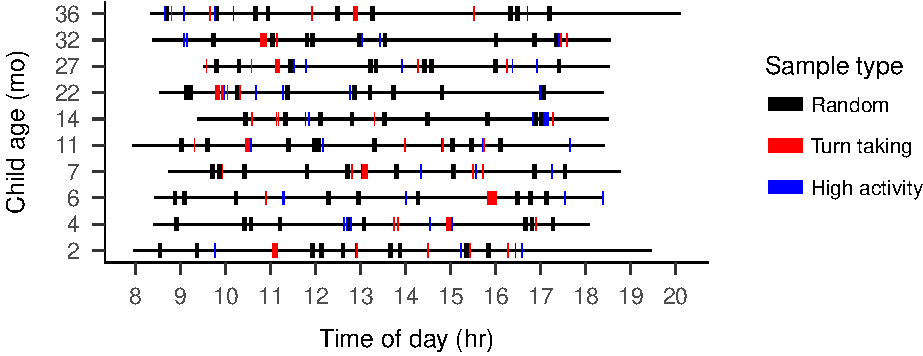
\includegraphics{Tseltal-CLE_files/figure-latex/fig0-1.pdf} Each video
clip was transcribed and annotated in ELAN (REFS) using the ACLEW
Annotation Scheme (REFS) by the first author and a native speaker of
Tseltal who lives in the community and knows most of the recorded
families personally. At the time of writing, NN\% \emph{{[}TASK XX: Fill
in before submitting{]}} of the clips have been reviewed by a second
native Tseltal speaker. The annotations include the transcription of
(nearly) all hearable utterances in Tseltal, a loose translation of each
utterance into Spanish, vocal maturity measures of each target child
utterance (non-linguistic vocalizations/non-canonical babbling/non-word
canonical babbling/single words/multiple words), and addressee
annotations for all non-target-child utterances
(target-child-directed/other-child-directed/adult-directed/adult-and-child-directed/animal-directed/other-speaker-type-directed).\footnote{Full documentation, including training materials, for the ACLEW Annotation Scheme can be found at *[TASK 11: Add OSF link]*.}

\subsubsection{Why vocal maturity?}\label{why-vocal-maturity}

\emph{{[}TASK 12: Missing paragraph!!{]}}

\subsection{Data analysis}\label{methods-analysisinfo}

We exported each ELAN file as tab-separated values and then the
annotations into R version 3.5.0 (2018-04-23) for analysis (plots:
ggplot2; analyses: lme4 and betareg \emph{{[}TASK 13: Fix references to
packages and their citations{]}}). We then calculated a number of
summary variables to characterize children's language environments and
linguistic development including: the rate of all overheard speech
(\enquote{XDS}) and all speech directed to the target child
(\enquote{TCDS}) in both minutes per hour and utterances per hour, the
proportion of speech in TCDS and coming from adult vs.~child speakers,
the rate of target-child-to-other and other-to-target-child turn
transitions, the rate of vocalization produced by the target child, and
the average maturity of children's vocalizations. Using language
environment measures from the turn-taking sample, we then also estimated
the number of intensive interaction minutes each child experienced over
the day.

\section{Results}\label{results}

\subsection{Speech quantity}\label{speech-quantity}

How much speech do Tseltal children hear overall and what proportion of
that speech is directed to them? For maximum comparability with prior
work we first limit direct comparisons to the randomly sampled Tseltal
clips. During randomly sampled clips, Tseltal children heard an average
of 24.68 minutes of speech per hour (median = 20.12; range =
8.23--48.60), of which an average of 3.63 minutes were directed toward
the target child (median = 4.08; range = 0.83--6.55). Consequently, the
mean proportion of speech directed to children was 0.29 (median = 0.28;
range = 0.05--0.77). By-child estimates of the overheard speech
(other-directed speech; \enquote{ODS}) rate, target-child-directed
speech (\enquote{TCDS}) rate, proportion TCDS (TCDS/(TCDS+ODS)), and
TCDS rate from adult vs.~child caregivers are shown in
\protect\hyperlink{fig1}{figure 1}. To these figures we have added
estimates from prior work with other
communities.\footnote{The Yucatec Mayan data from Shneidman and colleagues was originally reported in utterances per hour. We convert their estimates to minutes per hour using the median utterance duration in our dataset for all non-target child speakers (1029ms)}.

\begin{figure}
\centering
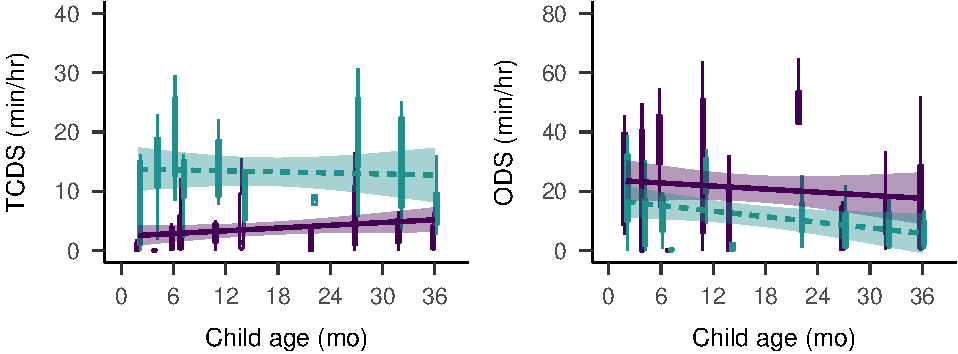
\includegraphics{Tseltal-CLE_files/figure-latex/fig1-1.pdf}
\caption{\label{fig:fig1}By-child estimates of minutes per hour of overheard
speech (upper left), target-child-directed speech (upper right),
proportion of speech that is directed to the target child (lower left),
and number of speakers present (lower right). Data are shown for the
random (purple; solid) and turn taking (green; dashed) samples. Bands on
the solid linear trends show 95\% CIs.}
\end{figure}

We modeled these measures for the nine clips from each child using
mixed-effects regression using the glmmTMB package in R (REF). Notably,
gaussian linear regression is not appropriate for any of our measures .
The rate-based dependent variables (ODS min/hr and TCDS min/hr) are
continuous with a zero-inflated positive distribution, the proportion
TCDS variable (TCDS/(TCDS+ODS)) is doubly-bounded, and the number of
speakers is count data (i.e., non-continuous).

To address this issue for the rate variables (ODS and TDS min/hr), we
rounded each rate estimate down to nearest minute per hour to treat it
as count data and then employed zero-inflated negative binomial
regression (ZINB). ZINB regressions model the dependent variable in two
ways: (1) a binomial (\enquote{zero-inflation}) model that evaluates the
likelihood that a datapoint is zero or non-zero and (2) a negative
binomial (\enquote{conditional}) model of all the non-zero datapoints
(REF). For proportion TCDS we used beta regression, which is suited to
making predictions on doubly-bounded data (for more details see Smithson
REFS).

Our primary predictors were as follows: child age, household size, and
number of non-target-child speakers present in that clip (all centered
and standardized), plus maternal education (pre-secondary
vs.~secondary-plus)\footnote{Spanish-only education begins in secondary school.},
and squared time of day at the start of the clip (in decimal hours;
centered on noon and standardized). We used squared time of day to model
the cycle of activity at home: mealtimes in the mornings and evenings
should be more similar to each other than the afternoon because of
dispersal for chores. To this we also added two-way interactions between
child age and maternal education, number of speakers, household size,
and time of day. Finally, we included a random effect of child, with
random slopes of time of day, unless doing so resulted in model
non-convergence. Finally, for the zero-inflation models of
zero-vs-nonzero ODS and TDS rate, we included household size, number of
speakers present, and time of day, with interactions between time of day
and household size and time of day and number of speakers present. The
zero-inflation models used the same random effects structure as their
complementary conditional models. We often had to reduce the fixed
effects structure in the zero-inflation model to achieve convergence, as
detailed below.

The quantity of other-directed speech (ODS) was primarily affected by
the number of speakers present (MODEL-REF): more speakers was associated
with more overheard speech. ODS was also significantly affected by time
of day, being more frequent in the mornings and evenings than around
midday (MODEL-REF). ODS was also more frequent in large households for
older children compared to younger children (MODEL-REF). There was no
significant effect of child age overall, and no effect involving
maternal education. The zero-inflation model of ODS included fixed
effects of household size, time of day, and their interaction, but none
of these predictors were significant.

The quantity of target-directed speech (TCDS) was primarily affected by
factors relating to the child's age. Older children heard more TCDS
(MODEL-REF) than younger children in general, particularly when many
other speakers were present (MODEL-REF). This also meant that, compared
to younger children, older children showed a much stronger effect of
time of day: younger children tended to hear a stable quantity of TCDS
throughout the day while older children heard much more TCDS in the
mornings and evenings compared to midday (MODEL-REF). The zero-inflation
model of TCDS also showed significant effects of house size, time of
day, and the interaction of time of day and number of speakers; TCDS is
more likely to be present in smaller households (MODEL-REF) and in the
mornings and evenings (MODEL-REF), particularly when there are more
speakers present (MODEL-REF).

As reviewed above, previous work on Mayan communities, including the
Tseltal community suggests that Mayan children hear much TCDS from other
children, and that the proportion of TCDS from other children increases
with age (REFS). In order to analyze the effect speaker age (child or
adult TCDS) together with the other predictors modeled above, we split
the data into TCDS from adults and children. All other predictors
remained the same, only the number of speakers present represented the
number of speakers of the relevant type for that datapoint (i.e.,, TCDS
rate from adults in clip 1 given the number of adult speakers present in
clip 1).

The quantity of TCDS was strongly affected by speaker age: in contrast
to prior work, these data show that most TCDS comes from adults
(MODEL-REF). In addition, this model replicates the interaction between
child age and time of day: older children hear most of their TCDS in the
mornings and evenings while younger children hear stable TCDS over the
day (MODEL-REF). We also find that speaker age effects depend on how
many speakers there are of each type: while TCDS form children is more
likely when more children are present, adults do not show a similar
effect (MODEL-REF). The zero-inflation model of TCDS from adults and
children included fixed effects of household size, time of day, and
their interaction, but none of these predictors were significant.

The overall proportion of speech directed to the child (proportion TCDS)
decreased when more speakers were present (MODEL-REF). Despite this,
older children still showed a stronger time of day effect than younger
children, with proportionally more TCDS in the mornings and evenings
(MODEL-REF). There were no significant overall effects of age, nor were
there any effects of maternal education or household size on the
proportion of TCDS used.

\subsubsection{Speech quantity during peak
moments}\label{speech-quantity-during-peak-moments}

Children's linguistic experiences are bursty (REFS) and, as we have
seen, speech is distributed asymetrically throughout the day in Tseltal
children's environments. If, for example, children do most of their
language learning for the day during these short bouts of interaction,
it may be more useful to characterize their learning environment with
respect to the interactional periods---what kinds of speech do they hear
during interaction?---rather than averaging over the entire day. We
therefore repeat the same set of analyses with the turn-taking subset of
the child's data: ODS rate, TCDS rate, TCDS rate by speaker age, and
proportion TCDS.

During high turn-taking clips, Tseltal children heard an average of
25.21 minutes of speech per hour (median = 23.99; range = 12.94--38.29),
of which an average of 13.28 minutes were directed toward the target
child (median = 13.65; range = 7.32--20.19). Consequently, the mean
proportion of speech directed to children was 0.62 (median = 0.62; range
= 0.37--0.93).

Using the same approach as before, we modeled the four speech quantity
measures for the 5--6 turn-taking
clips\footnote{The turn-taking clips included in this analysis are: the five 1-minute turn-taking clips and also the 5-minute 'extension' clip for that recording if it was an extension of a turn-taking clip}
from each recording.

As in the random sample, when more speakers were present, ODS was
significantly more frequent (MODEL-REF). While time of day significantly
affected ODS rate in the random sample, its effect on the turn-taking
bouts was only marginal, and trended in the opposite direction, i.e.,
more overheard speech during afternoon turn-taking bouts (MODEL-REF).
Furthermore, there was no evidence of interactions between time of day
and household size, as there was in the random sample. The
zero-inflation model included fixed effects of household size, time of
day, and their interaction, but none of these predictors were
significant.

The only significant factor affecting TCDS quantity in the turn-taking
sample was a two-way interaction between child age and time of day
(MODEL-REF). In contrast to the random sample this interaction showed
that younger children hear more TCDS during morning and evening
turn-taking bouts, but TCDS is more uniform across the day in older
children's turn-taking bouts. Unlike the random sample, this turn-taking
sample showed no main effect of child age: older and younger children
heard comparable amounts of TCDS overall. There was also no significant
interaction between age and number of speakers present, like there was
in the random sample. The zero-inflation model included fixed effects of
household size, time of day, and number of speakers, plus two-way
interactions of time of day and household size, and time of day and
number of speakers present. While, in the random sample, clips with
no-vs-some TCDS were significantly predicted by house size, time of day,
and the interaction of time of day and number of speakers, none of these
factors significantly predicted the presence of TCDS in the turn-taking
clips.

The model of TCDS quantity by speaker age for the turn-taking sample
showed some similar results to the random sample. First, the quantity of
TCDS in the turn-taking sample was strongly affected by speaker age
(MODEL-REF) due to the fact that most TCDS still came from adults.
Second, the presence of more children increased the quantity of TCDS
from children more than the presence of more adults increased the
quantity of TCDS from adults (MODEL-REF). However, TCDS quantity by
speaker in the turn taking data also showed an inverse effect of time of
day and child age, compared to that found in the randomly sampled data:
TCDS was maximized during turn-taking bouts that took place in the
mornings and evenings for younger children, but more uniform throughout
the day for older children (MODEL-REF).

In addition, the turn-taking bouts also showed a significant effect of
number of speakers: more speakers was associated with less TCDS
(MODEL-REF). There was also an interaction between child age and speaker
age: older children heard an increasing amount of TCDS from other
children during turn-taking bouts (MODEL-REF). The zero-inflation model
of TCDS from adults and children included fixed effects of household
size, time of day, and their interaction, but none of these predictors
were significant.

As in the random sample, the overall proportion of speech directed to
the child (proportion TCDS) decreased when more speakers were present
(MODEL-REF). Unlike the random sample, however, there was no interaction
between child age and time of day. There were no other significant
predictors of proportion of speech in TCDS.

\subsection{Interactional exchanges}\label{interactional-exchanges}

We can also measure children's linguistic environments as a summary of
the interactional exchanges they partake in (see also Romeo REFS). When
children are jointly engaged with an interlocutor, they can practice
making contingent vocalizations, and both the child and the interlocutor
can more easily coordinate their behaviors and social and communicative
intentions. We characterize children's interactional exchanges with four
measures: the rate of child-to-other turn transitions, other-to-child
turn transitions, the average duration of interactional sequences, and
the ratio of interlocutor vs.~child vocalization time. We first describe
these measures with respect to the random sample then, for comparison,
examine the turn-taking sample.

\begin{figure}
\centering
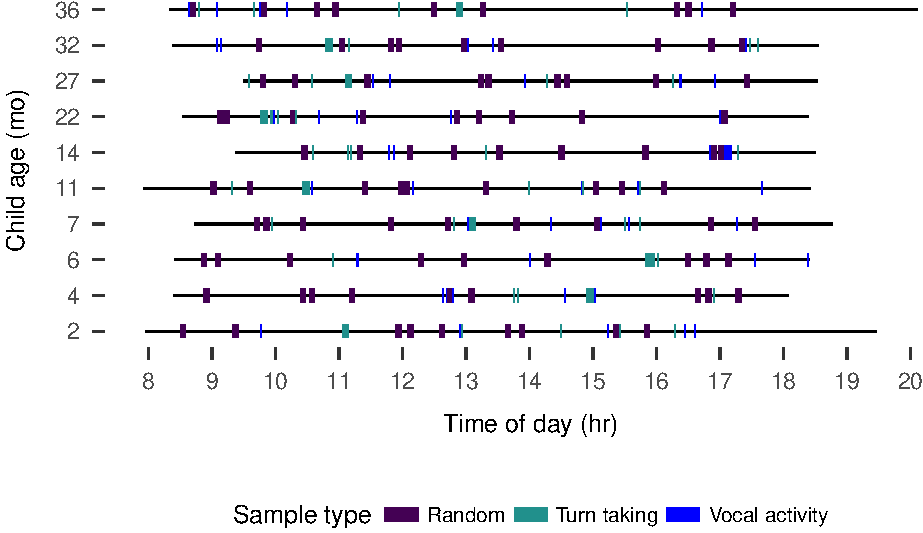
\includegraphics{Tseltal-CLE_files/figure-latex/fig2-1.pdf}
\caption{\label{fig:fig2}By-child estimates of minutes per hour of
child-to-other (upper left) and other-to-child (upper right) turn
transitions per minute, turn-taking sequenec duration (lower left), and
normalized difference in vocalization time (1 = child vocalizes more
than their interlocutor; 0 = vice versa). Data are shown for the random
(purple; solid) and turn taking (green; dashed) samples. Bands on the
solid linear trends show 95\% CIs}
\end{figure}

Details about models here

\subsubsection{Interactional exchanges during peak
moments}\label{interactional-exchanges-during-peak-moments}

\subsection{Frequency of high turn-taking
activity}\label{frequency-of-high-turn-taking-activity}

\begin{figure}
\centering
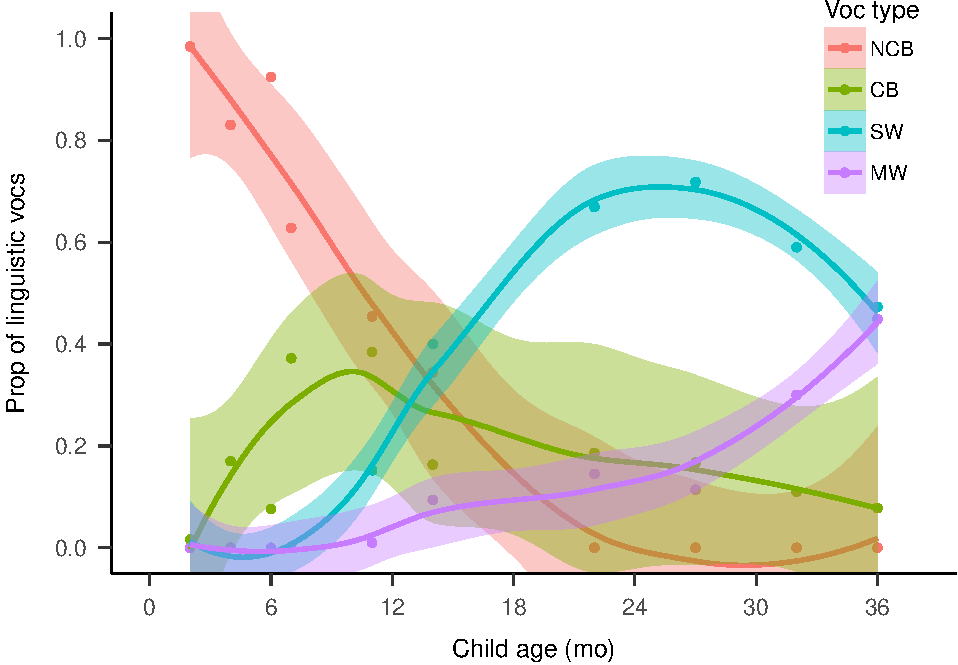
\includegraphics{Tseltal-CLE_files/figure-latex/plot_chi_voctypes_overall-1.pdf}
\caption{}
\end{figure}

\begin{verbatim}
## Warning in bind_rows_(x, .id): binding factor and character vector,
## coercing into character vector
\end{verbatim}

\begin{verbatim}
## Warning in bind_rows_(x, .id): binding character and factor vector,
## coercing into character vector
\end{verbatim}

\begin{verbatim}
## Warning in bind_rows_(x, .id): binding factor and character vector,
## coercing into character vector
\end{verbatim}

\begin{verbatim}
## Warning in bind_rows_(x, .id): binding character and factor vector,
## coercing into character vector
\end{verbatim}

\section{Discussion}\label{disc}

\subsection{Future directions}\label{disc-future}

\subsection{Conclusion}\label{disc-conclusion}

\section{Acknowledgements}\label{acknowledgements}

\newpage

\section{References}\label{refs}

\begingroup
\setlength{\parindent}{-0.5in} \setlength{\leftskip}{0.5in}

\hypertarget{refs}{}

\endgroup






\end{document}
